\chapter{Analysis of oscillatory time series}
\label{ch:analysis}

% Introduction: overview of the 'pipeline'
\section{Overview}
\label{sec:analysis-overview}

% - Zielinski et al. (2014) is a good starting point
% - Titles of the section lends themselves to a punchy opener paragraph that
%   describes the process

% From synthetic oscillations report
In the time series analysis literature, there is a wealth of analysis methods that aim to find parameters pertaining to the periodicity of noisy time series and that aim to characterise the relationship between two signals.
This is relevant for biological time series, especially because they are noisy due to both intrinsic and extrinsic noise sources, and because researchers often record multiple time series from the same system to study the relationship between such time series.
One example is the yeast metabolic cycle, which is known to be a metabolic oscillator that is coupled with the cell division cycle oscillator -- in this case, the two time series from this system consist of the level of metabolites to represent the metabolic oscillator and the activity of a component of the cell division cycle to represent the cell division cycle.

The problem with applying classical time series analysis methods to biological time series lies with two properties of biological time series: they are noisy and they are often short.
Classical methods such as Fourier analysis have been shown to be useful in characterising noisy biological time series when they are long, e.g. from neuron impulse recordings, which can include up to thousands of oscillations.
However, for examples such as the yeast metabolic cycle, it is not feasible to record time series that include such a high number of oscillations; in this case, 5-10 oscillations are more realistic.
As a result, methods like Fourier analysis only provide poor resolution for characteristics such as the period of oscillations.

\section{Cleaning: choosing data, filtering, missing time points}
\label{sec:analysis-cleaning}

\section{Classification: is my time series oscillatory?}
\label{sec:analysis-classification}

% Literature review subsection
\subsection{Rhythmicity detection for biological data}
\label{subsec:analysis-classification-rhythmicity}
% - Compare and contrast methods
% - Highlight challenges with large datasets of noisy biological data
% - Review existing methods first and then talk about the methods I tried, with results.

% Copied from 10m report
% ----------------------
% Minireview of studies about finding whether there is an oscillation in circadian time series (or other related time series) -- keep it relatively short.

% Discussion about oscillatory behaviour vs periodic behaviour?

To assess how a perturbation affects the YMC, it is important to have a systematic method to determine whether a time series is oscillatory.
\citet{glynnDetectingPeriodicPatterns2006} describe a method to classify gene expression profiles as oscillating or non-oscillating based on the Lomb-Scargle periodogram \citep{lombLeastsquaresFrequencyAnalysis1976}.
This periodogram was developed for time series with missing time points, and has a chi-square distribution that aids a statistical test for periodicity \citep{scargleStudiesAstronomicalTime1982}.
The classification was based on controlling the false discovery rate for identification of oscillations.
In testing multiple hypotheses, the false discovery rate is defined as the proportion of cases in which the null hypothesis is true among all hypotheses in which the test is declared significant.
Increasing the false discovery rate thus increases the proportion of time series classed as oscillating.

I developed a classifier based on \citet{glynnDetectingPeriodicPatterns2006} to classify time series of flavin autofluorescence.
%I then compared the classification results against manual classification of these time series into oscillating and non-oscillating.
The classifier was able to rank the time series by quality of oscillation (figure \ref{fig:ClassifierBestWorstTS}).
The peak of the normalised classical periodogram of each time series was used as a proxy for the quality of oscillation (figure \ref{fig:ClassifierBestWorstPS}).
By eye, birth events coincided with peaks of some higher-quality oscillations.
However, this was also true for some oscillations ranked as lower-quality.
% [COMMENTED -- don't think this sentence is really consequential, and the proposed plot doesn't add much] Additionally, higher-quality oscillations do not seem to be associated with imaging positons/flavin LED exposure times. % FIGURE: scatter plot, horizontal axis is rank, vertical axis is imaging position
% Wee bit of discussion (plus a plot to illustrate my point).  Deeper discussion about multiple main frequencies is in discussion, and has references to literature.
These oscillations were ranked as low-quality because the Fourier transform identified multiple main frequencies, and thus lowered the peak of the normalised periodogram.
Thus, a Fourier-based method may not adequately provide the information for a reliable ranking of oscillation quality.

\begin{figure}[htbp]
  \centering
  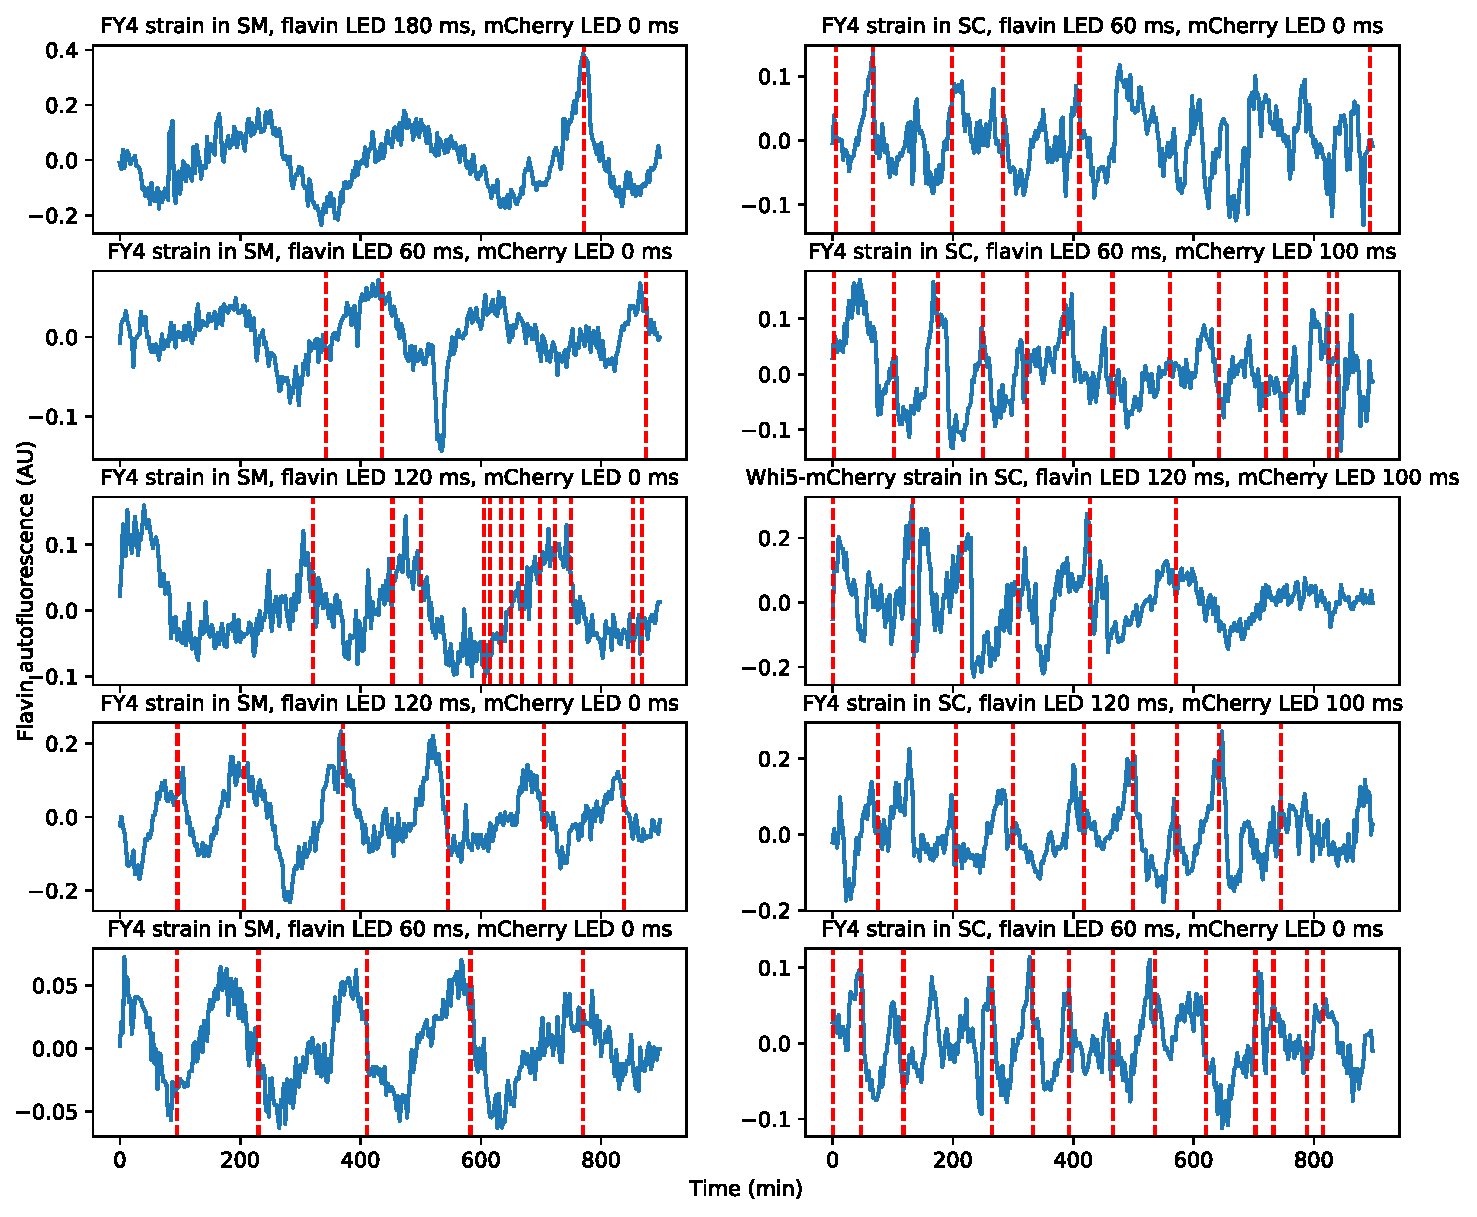
\includegraphics[width=\textwidth]{10m_ClassifierBestWorstTS}
  \caption{Classifier ranks time series by quality of oscillation.
    Left column shows `best' five and right column shows `worst' five.
    Blue: flavin autofluorescence, red: automatically identified birth}
  \label{fig:ClassifierBestWorstTS}
\end{figure}

\begin{figure}[htbp]
  \centering
  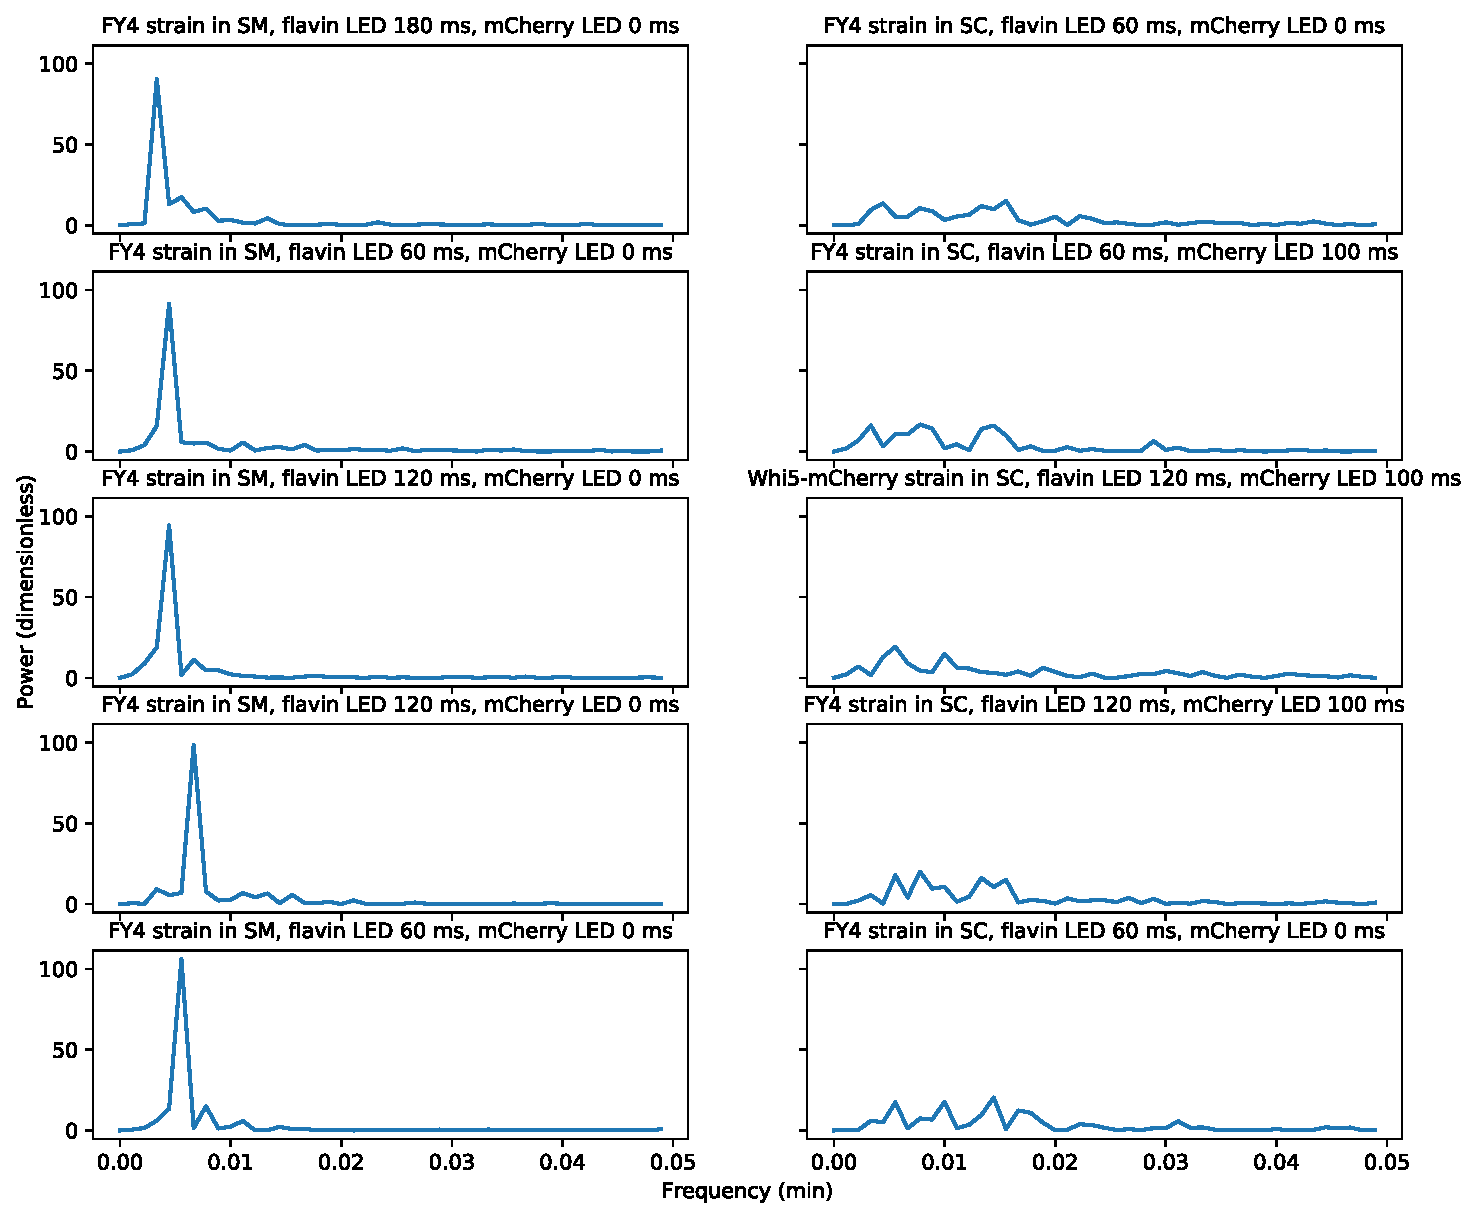
\includegraphics[width=\textwidth]{10m_ClassifierBestWorstPS}
  \caption{Highest peak of normalised classical periodograms is an inadequate proxy for quality of oscillations.
    Lines: normalised classical periodograms of time series in figure \ref{fig:ClassifierBestWorstTS}.}
  \label{fig:ClassifierBestWorstPS}
\end{figure}


\subsection{Machine learning approaches to classification}
\label{subsec:analysis-classification-ml}
% - Write results from classifier project (SVM, RF, etc.)

% Copied from 10m report...
% Note: this predates the classifier project --
% I now have better data, understand ML more, and have better methods.
% However, I still think it's instructive in writing an 'update' when I read all the content together
% ----------------------
% ROC: DISCUSS IN PRESENTATION AS AN APPENDIX SLIDE
% also re-word. I wrote this when I was tired.
Currently, the oscillation classifier has limited use.
It is difficult to characterise the time series of flavin autofluorescence using standard methods based on the data available.
The peak of the normalised classical periodogram inadequately captures the quality of the oscillations.

The oscillation classifier has one tuning parameter, the false discovery rate, and its value affects the proportion of time series classed as oscillating.
A reliable ground truth is needed to optimise the value of the false discovery rate so that the classification accuracy is maximised.
Because none of the experiments performed were ones from which oscillations were not expected, I lacked a reliable ground truth for the presence of oscillations.
I resorted to subjective judgements of whether a time series exhibited oscillations, and thus any optimised false discovery rate would have low reliability.

The YMC gene deletion experiments discussed in section [REF: SYNCHRONY SECTION FROM 10m] will provide a more reliable ground truth for the development of the oscillation classifier, as oscillations are not expected in these experiments.
%Furthermore, I will construct neural net-based classifiers so that more information is leveraged from the time series to inform the classifier.
With the improved ground truth, I will then compare the performance of the oscillation classifier with graph-based clustering in discriminating between oscillating and non-oscillating time series.

\section{Characterisation: I have one time series -- what properties does it have?}
\label{sec:analysis-characterisation}

% Literature review subsection
\subsection{Periods, phases, amplitudes}
\label{subsec:analysis-characterisation-quantities}

\subsection{Combining methods to get a picture of periodicity}
\label{subsec:analysis-characterisation-combined}


\section{Clustering: I have many time series (of the same signal) from many cells -- what are their relationships to each other?}
\label{sec:analysis-clustering}

% Literature review subsection
\subsection{(Literature)}
\label{subsec:analysis-clustering-literature}

\subsection{Machine learning approaches to clustering}
\label{subsec:analysis-clustering-ml}
% - Featurisation -- decisions to make
% - Clustering approaches and algorithms -- compare and contrast
% - Review existing methods first and then talk about the methods I tried, with results.

% Copied from 10m report
% ----------------------
Graph-based Clustering of Oscillations Based on Feature Vectors
%\label{sec:graphclustering}

% mini-review -- IT'S PRETTY UNWIELDY AT THIS POINT, AND REFERENCES CONCEPTS NOT DISCUSSED TILL LATER
Clustering of time series has been used to identify groupings within a set of time series \citep{wangStructureBasedStatisticalFeatures2007}, including biological time series \citep{shafieiDopamineSignalingModulates2019}, or even transcript cycling patterns in YMCs \citep{tuLogicYeastMetabolic2005}.
However, \citet{wangStructureBasedStatisticalFeatures2007} and \citet{tuLogicYeastMetabolic2005} employed $k$-means clustering, which requires the user to specify the number of clusters, and therefore may not reflect the underlying structure of the set of time series.
Though \citet{shafieiDopamineSignalingModulates2019} used modularity clustering \citep{newmanModularityCommunityStructure2006}, the method was based on one time series feature, which may not adequately capture the characteristics of the time series.

Thus, I converted each time series of flavin autofluorescence to a vector of features, and represented the vectors as nodes on a geometric graph.
Such a geometric graph may function as a visualisation tool as well.

% FIGURE: pipeline and options.  It's rather difficult to visualise what happens, so such a figure, like the one I often use in the lab presentations in the summer, will be helpful.  Though may be more impactful in the presentation rather than in this report.

\subsubsection{Supervised Classification}
\label{sec:graphclustering-supervised}

I employed the \emph{hctsa} toolbox \citep{fulcherHctsaComputationalFramework2017} to compute vectors of features for each time series.
This toolbox contains 7701 features defined from across the time series analysis literature.
I focused on the 22-feature \emph{catch22} subset of the original 7701 features (table \ref{tab:catch22}).
\citet{lubbaCatch22CAnonicalTimeseries2019} selected these 22 features because they minimise redundancy while maintaining classification performance across 93 test datasets.
This feature set excludes features that are dependent on mean or spread.

% sort these by accuracy. (jesus christ this looks like a fuckload of work...)
\begin{table}[htbp]
  \small
  \centering
  \begin{tabularx}{\linewidth}{bbS}
    % To do: make numbers align right.  Also I'm not really sure if should be putting the accuracies here when I have them in a violin plot...
    \toprule
    Feature name & Description & Accuracy\\
    \midrule
    \texttt{DN\_\-HistogramMode\_\-5} & Mode of z-scored distribution (5-bin histogram) &  46.43 \\
    \texttt{DN\_\-HistogramMode\_\-10} & Mode of z-scored distribution (10-bin histogram) & 53.15 \\
    \texttt{SB\_\-BinaryStats\_\-mean\_\-longstretch1} & Longest period of consecutive values above the mean  & 66.47 \\
    \texttt{DN\_\-OutlierInclude\_\-p\_\-001\_\-mdrmd} & Time intervals between successive extreme events above the mean & 57.80 \\
    \texttt{DN\_\-OutlierInclude\_\-n\_\-001\_\-mdrmd} & Time intervals between successive extreme events below the mean & 56.45 \\
    \texttt{first\_\-1e\_\-ac} & First 1/e crossing of autocorrelation function & 78.97 \\
    \texttt{firstMin\_\-acf} & First minimum of autocorrelation function & 81.96 \\
    \texttt{SP\_\-Summaries\_\-welch\_\-rect\_\-area\_\-5\_\-1} & Total power in lowest fifth of frequencies in the Fourier power spectrum & 60.57 \\
    \texttt{SP\_\-Summaries\_\-welch\_\-rect\_\-centroid} & Centroid of the Fourier power spectrum & 81.41 \\
    \texttt{FC\_\-LocalSimple\_\-mean3\_\-stderr} & Mean error from a rolling 3-sample mean forecasting & 71.73 \\
    \texttt{CO\_\-trev\_\-1\_\-num} & Time-reversibility statistic, $\langle(x_{t+1} - x_t)^3\rangle_t$ & 65.42 \\
    \texttt{CO\_\-HistogramAMI\_\-even\_\-2\_\-5} & Automutual information, $m = 2, \tau = 5$ & 77.01 \\
    \texttt{IN\_\-AutoMutualInfoStats\_\-40\_\-gaussian\_\-fmmi} & First minimum of the automutual information function & 75.85 \\
    \texttt{MD\_\-hrv\_\-classic\_\-pnn40} & Proportion of successive differences exceeding $0.04\sigma$ & 47.05 \\
    \texttt{SB\_\-BinaryStats\_\-diff\_\-longstretch0} & Longest period of successive incremental decreases & 55.69 \\
    \texttt{SB\_\-MotifThree\_\-quantile\_\-hh} & Shannon entropy of two successive letters in equiprobable 3-letter symbolization & 49.63 \\
    \texttt{FC\_\-LocalSimple\_\-mean1\_\-tauresrat} & Change in correlation length after iterative differencing & 76.07 \\
    \texttt{CO\_\-Embed2\_\-Dist\_\-tau\_\-d\_\-expfit\_\-meandiff} & Exponential fit to successive distances in 2-d embedding space & 62.65 \\
    \texttt{SC\_\-FluctAnal\_\-2\_\-dfa\_\-50\_\-1\_\-2\_\-logi\_\-prop\_\-r1} & Proportion of slower timescale fluctuations that scale with DFA (50\% sampling) & 59.34 \\
    \texttt{SC\_\-FluctAnal\_\-2\_\-rsrangefit\_\-50\_\-1\_\-logi\_\-prop\_\-r1} & Proportion of slower timescale fluctuations that scale with linearly rescaled range fits & 72.54 \\
    \texttt{SB\_\-TransitionMatrix\_\-3ac\_\-sumdiagcov} & Trace of covariance of transition matrix between symbols in 3-letter alphabet & 57.40 \\
    \texttt{PD\_\-PeriodicityWang\_\-th0\_\-01} & Periodicity measure of \citet{wangStructureBasedStatisticalFeatures2007}   & 68.32 \\
    \bottomrule \\
  \end{tabularx}
  \caption{\emph{catch22} features, adapted from \citet{lubbaCatch22CAnonicalTimeseries2019}.
  The accuracies (\%) of the linear classifiers based on each feature, tasked to discriminate between cells grown in SC and cells grown in SM, are indicated.}
  \label{tab:catch22}
\end{table}

%----- SC VS SM -----
%I found that \emph{catch22} features have a varied ability to distinguish experimentally relevant groupings in the dataset. %; however, this may be attributed in part to the limitations of the experiments.  % strong link to discussion --> what experiments to do to rectify this
Feature extraction was able to discriminate between cells grown in complete and minimal media.
A linear support vector machine (SVM) trained on the 22-element feature vectors was able to classify the two groups with a mean accuracy of 76.67\%, using 10-fold cross validation.
For comparison, the accuracy of random guessing is 50.00\%.
This classification performance can be shown by a confusion matrix (figure \ref{fig:EffectofMediaCM}), which refers to a contingency table that shows the numbers of instances predicted to belong in each group in rows, and shows the numbers of instances in actual groups in columns.
Furthermore, \texttt{first\-Min\_\-acf} and \texttt{SP\_\-Sum\-ma\-ries\_\-welch\_\-rect\_\-cen\-troid} (table \ref{tab:catch22}) had the greatest linear classifier accuracies.
Cells in minimal media had greater \texttt{first\-Min\_\-acf} values than cells in complete media, and lower \texttt{SP\_\-Sum\-ma\-ries\_\-welch\_\-rect\_\-cen\-troid} values (figure \ref{fig:EffectofMediaTopFeatures}).
These values were consistent with cells in minimal media having longer oscillation periods (figure \ref{fig:catch22validation}).
These results suggest that the period was an important defining feature for the two groups of cells.

\begin{figure}[htbp]
  \centering
  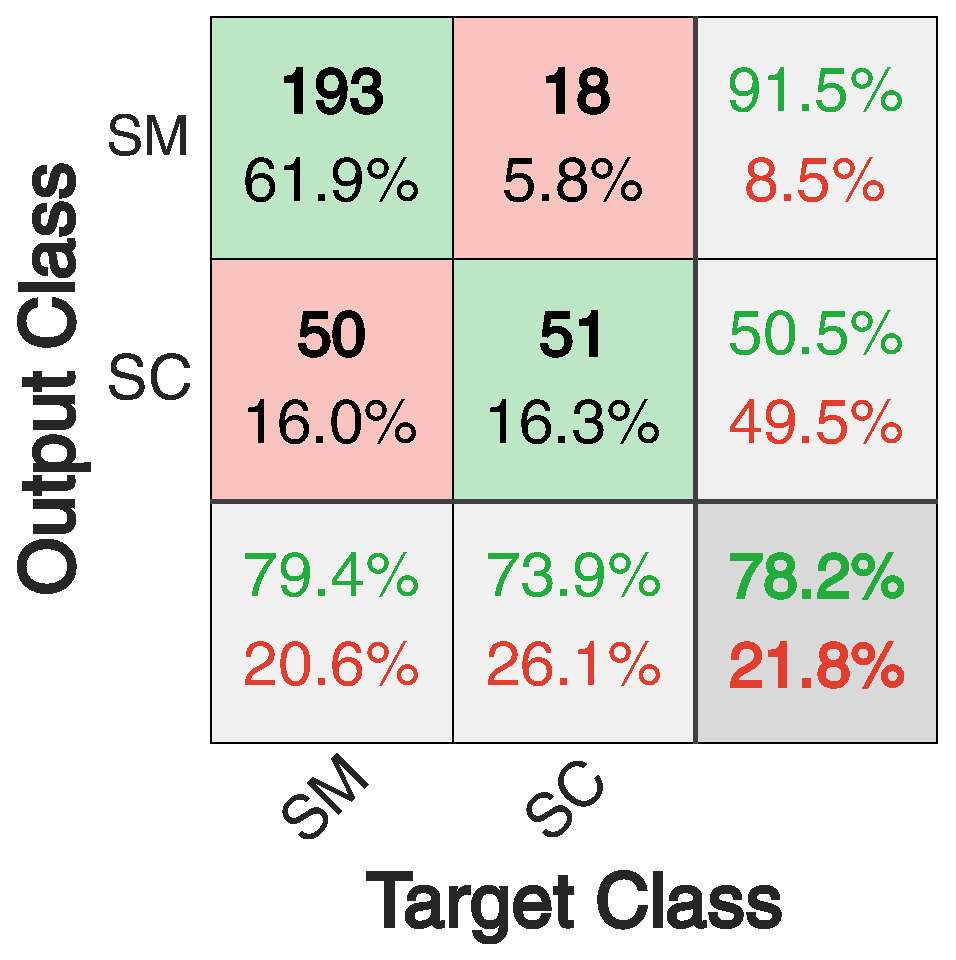
\includegraphics[width=0.3\textwidth]{10m_EffectofMediaCM}
  \caption{Linear support vector machine trained on \emph{catch22} features performed well at classifying cells cultured in complete (SC) and minimal (SM) media.
    Confusion matrix shows one out of ten repeats.
    For each row/column, green numbers indicate the proportion of correct identifications, and red numbers indicate the proportion of incorrect identifications.}
  \label{fig:EffectofMediaCM}
\end{figure}
% Remove top part of figure using Inkscape or something
% ideally I'd generate a figure in which less space is wasted, but I don't have the time now...

\begin{figure}[htbp]
  \centering
  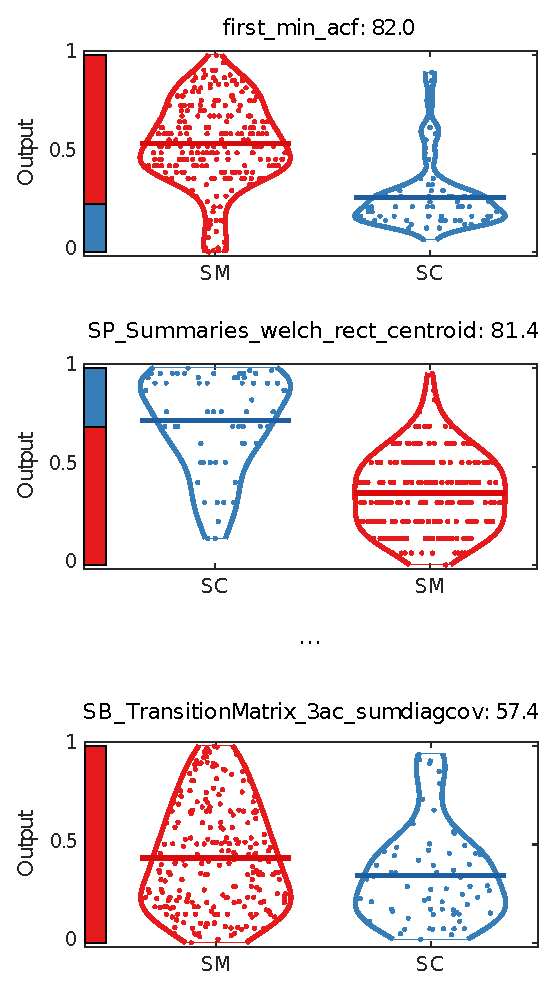
\includegraphics[width=0.45\textwidth]{10m_EffectofMediaTopFeatures}
  \caption{\texttt{first\-Min\_\-acf} and \texttt{SP\_\-Summaries\_\-welch\_\-rect\_\-centroid} performed best at classifying cells cultured in complete and minimal media because the distributions of feature values differed the most between the two groups.
    Numbers above violin plots indicate mean linear classification accuracy.}
  \label{fig:EffectofMediaTopFeatures}
\end{figure}
% might have to crop this

% :: BIG NEW FIGURE ::
\begin{figure}[htbp]
  \centering
  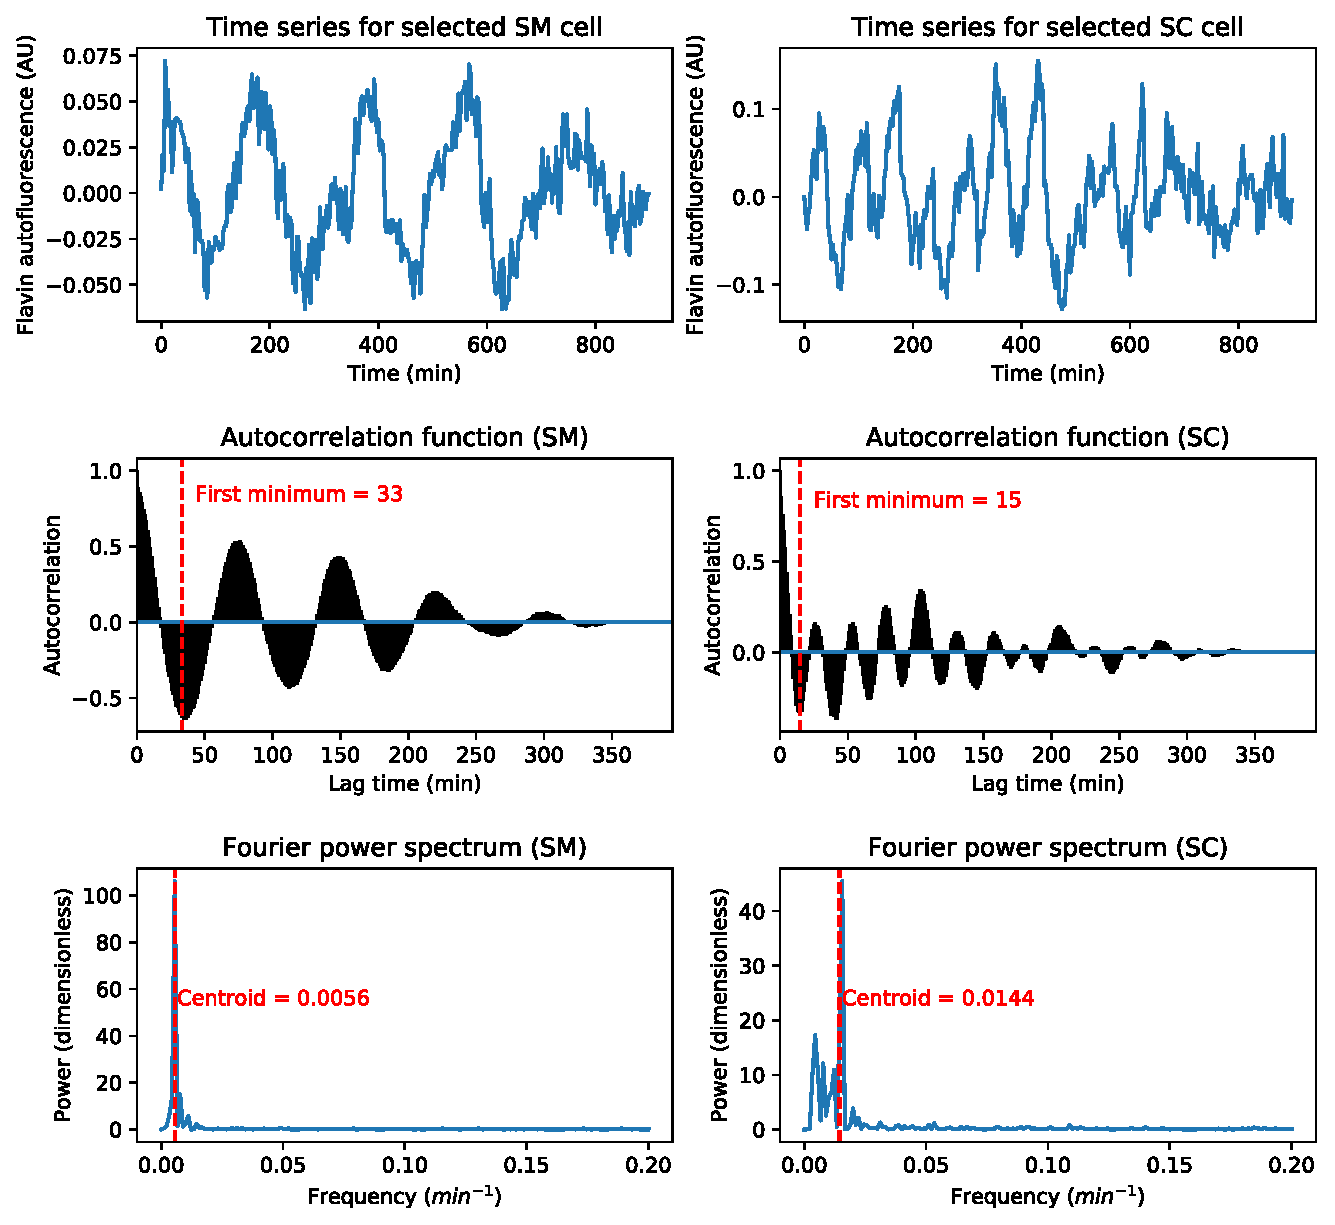
\includegraphics[width=\textwidth]{10m_catch22validation}
  \caption{Comparison of time series, autocorrelation function, and Fourier spectrum for a cell cultured in minimal media (SM) vs a cell cultured in complete media (SC)}
  \label{fig:catch22validation}
\end{figure}

%----- EXPOSURE TIME -----
In contrast, \emph{catch22} features performed poorly at discriminating between the three groups defined by flavin LED exposure time (\SI{60}{\milli\second}, \SI{120}{\milli\second}, \SI{180}{\milli\second}) in the set of cells cultured in complete media (SVM: 32.69\% accuracy, figure \ref{fig:FlavinExpostestCM}; accuracy of random guessing is 33.33\%).
% [I'm not sure if I should include this segue to using full-set hctsa.  I didn't mention it in the oscillating vs non-oscillating section.]
%With the full \emph{hctsa} feature set, the 25 features with the greatest mean linear classification accuracy in discriminating groups defined by exposure time were dependent on mean and spread.
%Having features that best distinguish the groups be dependent on mean and spread was consistent with cells subjected to longer exposure times exhibiting flavin signals of higher intensity %(mean raw readings for \SI{60}{\milli\second}: 0.63 AU, \SI{120}{\milli\second}: 1.3 AU, \SI{180}{\milli\second}: 1.7 AU;
%(standard deviations for time series from \SI{60}{\milli\second}: 0.040 AU, \SI{120}{\milli\second}: 0.067 AU, \SI{180}{\milli\second}: 0.085 AU). % is this needed?  is this too detailed?
These findings suggest that exposure time did not affect the characteristics of flavin autofluorescence traces apart from fluorescence intensity.

\begin{figure}[htbp]
  \centering
  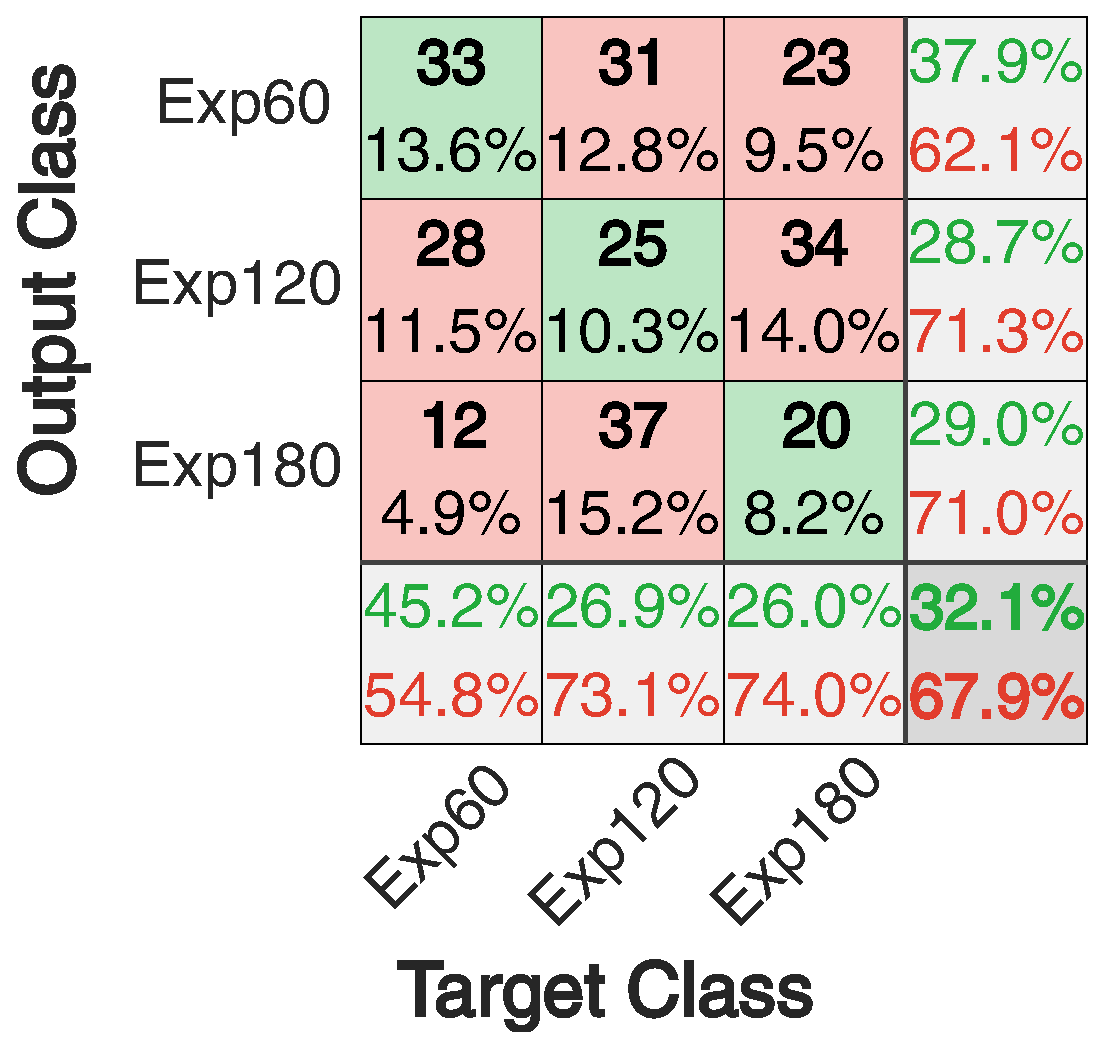
\includegraphics[width=0.4\textwidth]{10m_FlavinExpostestCM}
  \caption{Linear support vector machine trained on \emph{catch22} features performed poorly at classifying cells by LED exposure time.
    Confusion matrix shows one out of ten repeats.
    For each row/column, green numbers indicate the proportion of correct identifications, and red numbers indicate the proportion of incorrect identifications.}
  \label{fig:FlavinExpostestCM}
\end{figure}

%----- OSCILLATING VS NON-OSCILLATING -----

Discrimination between manually-categorised oscillating and non-oscillating flavin autofluorescence traces was also poor (SVM: 66.91\% accuracy, figure \ref{fig:OscillatingCM}; accuracy of random guessing is 50.00\%). %, and using the full \emph{hctsa} feature set was no better (SVM: XX.XX\% accuracy). % Add numbers.  (not sure of violin plots and confusion matrices will be very informative)
These results suggested that using 22 %or even 7700
features across disciplines did not improve on the oscillation classifier (section [INSERT REF HERE]), which was effectively based on one feature, namely, the peak of the normalised classical periodogram.

\begin{figure}[htbp]
  \centering
  \includegraphics[width=0.4\textwidth]{10m_OscillatingCM}
  \caption{Linear support vector machine trained on \emph{catch22} features performed poorly at classifying oscillating and non-oscillating time series.
    Confusion matrix shows one out of ten repeats.
    For each row/column, green numbers indicate the proportion of correct identifications, and red numbers indicate the proportion of incorrect identifications.}
  \label{fig:OscillatingCM}
\end{figure}

\subsubsection{Unsupervised Clustering}
\label{sec:graphclustering-unsupervised}

Modularity clustering is the problem of partitioning a graph into clusters in order to optimise a `modularity' value.
This value is defined as the number of edges between clusters minus the number of expected edges if edges are placed at random \citep{newmanModularityCommunityStructure2006}.
The general Louvain algorithm \citep{blondelFastUnfoldingCommunities2008,muchaCommunityStructureTimeDependent2010} is one method to solve this optimisation problem and define partitions for a graph.
This algorithm has a resolution parameter which specifies the scale of the clusters: low resolution gives large clusters, and high resolution gives small clusters \citep{fortunatoResolutionLimitCommunity2007}.

Unsupervised graph-based clustering suggested that the division between complete and minimal media was dominant among time series of flavin autofluorescence. %(figure \ref{fig:EffectofMediaClusters}).
I constructed an incomplete graph to represent the pairwise similarity between time series based on the \emph{catch22} feature vectors.
Then, I identified communities in the resulting network using the general Louvain algorithm.
When the resolution value was set so that the graph was partitioned into two clusters, the clusters conformed well to complete and minimal media groups (figure \ref{fig:EffectofMediaClusters}). % TABLE/NUMBER: Add a 'confusion matrix' (re-use code from 5m) and calculate accuracy (note: revert to some old commit to re-produce this -- why the hell did Fulcher have to change EVERYTHING ughhhhh).  Make clear the point that in each iteration, things are different.
% (this is the where the Rand value can be used instead, but there is no need -- just making a note here).
Such results suggested that unsupervised graph-based clustering may have potential to discover structure in the dataset.

\begin{figure}[htbp]
  \centering
  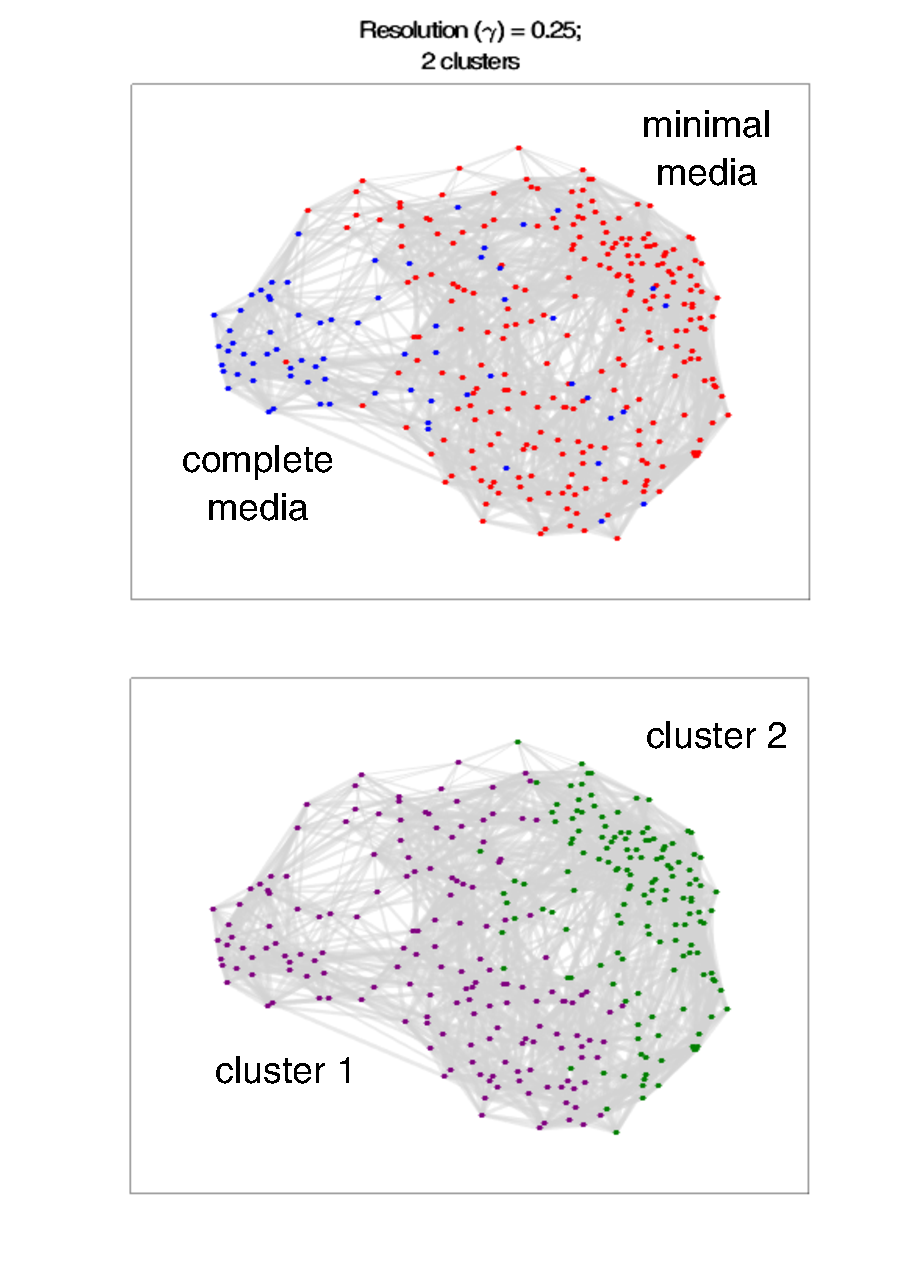
\includegraphics[width=0.5\textwidth]{10m_EffectofMediaClusters}
  \caption{Graph-based clustering partitions a geometric graph defined by pairwise cosine distances between \emph{catch22} vectors close to labels defined by media.}
  \label{fig:EffectofMediaClusters}
\end{figure}

Indeed, I found that the method was able to distinguish time series generated in my project from time series obtained by \citet{baumgartnerFlavinbasedMetabolicCycles2018} (figure \ref{fig:DistanceMatrixBaumgartner}, table \ref{tab:ClusterBaumgartner})
However, this ability to distinguish the data sources may have been because the data from different sources were processed in different ways.

\begin{figure}[htbp]
  \centering
  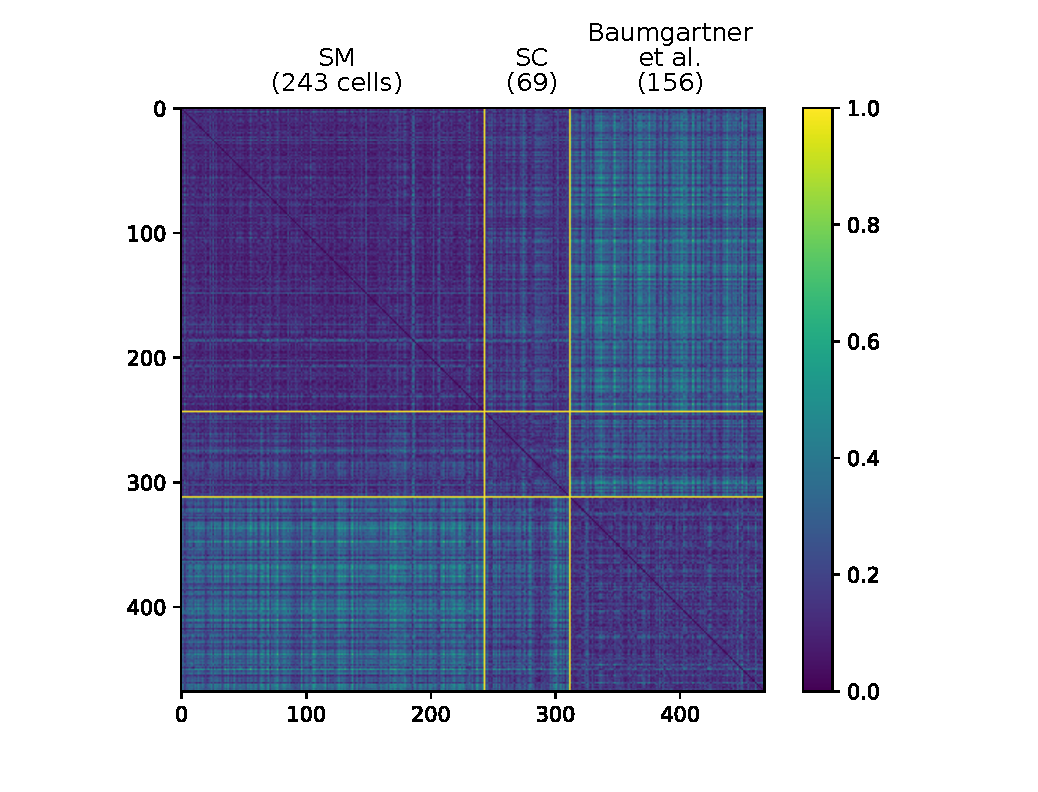
\includegraphics[width=0.6\textwidth]{10m_DistanceMatrixBaumgartner}
  \caption{Graph-based clustering was able to partition minimal media time series, complete media time series, and time series from \citet{baumgartnerFlavinbasedMetabolicCycles2018}.
    This distance matrix is based on cosine distances between \emph{catch22} feature vectors for pairs of time series.  Distances between 0 and 1 (legend, right) are represented as colours.}
  \label{fig:DistanceMatrixBaumgartner}
\end{figure}

\begin{table}[htbp]
  \centering
  \begin{tabular}[h]{rrrr}
    & SM & SC & Baumgartner et al.\\
    Cluster 1 & 1 & 11 & 141\\
    Cluster 2 & 63 & 28 & 6\\
    Cluster 3 & 56 & 22 & 8\\
    Cluster 4 & 79 & 4 & 0\\
    Cluster 5 & 44 & 4 & 1
  \end{tabular}
  \caption{Graph-based clustering is able to partition minimal media time series, complete media time series, and time series from \citet{baumgartnerFlavinbasedMetabolicCycles2018}.  Table shows one graph partition returned by the general Louvain algorithm.  The graph was constructed according to section [METHODS: HCTSA].  In this case, the default value for the resolution parameter was used.}
  \label{tab:ClusterBaumgartner}
\end{table}
% Rand index?

\section{Correlation: I have two signals from the same cell -- what are their relationships to each other?}
\label{sec:analysis-correlation}
% - Cross-correlation: start from the basic definitions, then extend to population-level cross-correlation as used by Kiviet et al. (2014)

% Copied from project: 'Modelling cross-correlation between sinusoids and relaxation oscillators',
% or, my 'synthetic oscillations report'.
% Currently doesn't really fit the thesis so much -- it comes with its own subsections, and this part can definitely be shorter.  Certainly, there shouldn't be a 'results' subsection.
This report explores the cross-correlation and autocorrelation functions, adapted to a population of noisy time series, as a method to characterise the periodicity and heterogeneity of oscillatory time series.  The report does so through simulated oscillatory time series based on models with very well-characterised behaviours: a harmonic oscillator and a relaxation oscillator.  The hope is that these synthetic time series can adequately model flavin fluorescence oscillations and the behaviour of histones during the cell division cycle.

\subsection{Mathematical basis}
\label{sec:analysis-correlation-maths}
\subsubsection{Simulating oscillators}
\label{sec:analysis-correlation-maths-osc}

I choose the harmonic oscillator and the FitzHugh-Nagumo model to investigate because they are simple, well-characterised, and mimic the biological time series that I am interested in.  Here I detail the rationale behind my choices and describe the oscillators I choose.

\begin{enumerate}
\item Harmonic oscillator
\label{sec:org7f23d98}

I choose the harmonic oscillator because it is the simplest case of an oscillator, with only one parameter.  Namely:

\(\frac{d^{2}y}{dt^{2}} = -\omega^{2}y\)

where \(y\) represents displacement and \(\omega\) represents the angular frequency.

Or written in the form of a system of first-order differential equations:

\(\frac{dy}{dt} = v\)

\(\frac{dv}{dt} = -\omega^{2}y\)

This model produces time series \(y(t)\) that is a sinusoid, i.e.

\(y(t) = A sin(\omega{}t + \phi)\)

where \(A\) and \(\phi\) are determined by initial conditions.

\item FitzHugh-Nagumo model
\label{sec:orgdffb616}

I choose the FitzHugh-Nagumo model because it is a well-characterised relaxation oscillator that can model a more complicated time series, while still being simple, with only four parameters.

The FitzHugh-Nagumo model was developed to model an excitable system, such as a neuron.  The model is described as a system of first-order differential equations (citation needed):

\(\frac{dv}{dt} = v - \frac{v^3}{3} - w + RI_{\mathrm{ext}}\)

\(\tau \frac{dw}{dt} = v + a - bw\)

where the variables include:
\begin{description}
\item[{\(v\)}] membrane voltage
\item[{\(w\)}] linear recovery variable
\end{description}

and the parameters include \(RI_{\mathrm{ext}}\) (external stimulus), \(\tau\), \(a\), and \(b\) [describe what they are and how they control the model].

This model produces time series \(v(t)\) that is a relaxation oscillator [why relaxation oscillator?].
\end{enumerate}

\subsubsection{Generating noise}
\label{sec:analysis-correlation-maths-noise}

Biological time series, and certainly the ones that I study, have noise.  So, it makes sense to add noise to our models as well, because noise affects the behaviour of models and the analysis methods applied to the time series generated by our models.

Here, I describe two types of noise I investigate and how to integrate them with my models.

\begin{enumerate}
\item Gaussian noise
\label{sec:org38e563f}

[To clarify: should I use white noise or Gaussian noise?  These are not equivalent, but can overlap.  Current code generates Gaussian noise.]

I use (white) Gaussian noise as it is the simplest, first-approach case.  This noise is generated by randomly drawing samples from the normal distribution \(\mathcal{N}(1,0)\).

[Figure may be useful, but only to contrast with Gillespie noise.]

\item Gillespie noise from birth-death process
\label{sec:orge5d486b}

I use Gillespie noise because it's the same type of noise from biological systems [citation needed, maybe Wilkinson `Stochastic Modelling for Systems Biology'].

The Gillespie noise was generated as follows, using example parameter values:

Define the birth-death process: birth rate \(k_{0} = 5\) and death rate \(d_{0} = 0.05\).  Set a stochastic simulation with final time of 1500, and put the trajectories on a grid with regularly-spaced time points, 1000 time points in this case.

Each trajectory took some time to reach steady state (see image below), so the latter half was taken, assuming it is in steady-state:
\begin{center}
\includegraphics[width=.9\linewidth]{gillespie.png}
\end{center}

Here, the steady-state mean is equal to the steady-state variance, which is equal to \(k_{0}/d_{0}\).

I normalised this trajectory by subtracting the mean (\(k_{0}/d_{0}\)) and then dividing by \(\sqrt{1/d_{0}}\) to create Gillespie noise with mean 0 and standard deviation \(\sqrt{k_{0}}\) -- this is so that changes in \(k_{0}\) affect the noise amplitude.

As an example, I show 3 trajectories of Gillespie noise using the initial parameters I set:
\begin{center}
\includegraphics[width=.9\linewidth]{gillespie_noise_samples.png}
\end{center}

Alternatively, Gillespie noise can be parametrised in the form of standard deviation of noise amplitude \(A = \sqrt{k_{0}/d_{0}}\) and noise timescale \(\tau = 1/d_{0}\).

\item Adding noise
\label{sec:org03ea61a}

Approach: add to time series (simple sum).
\end{enumerate}

\subsubsection{Computing autocorrelation and cross-correlation}
\label{sec:analysis-correlation-maths-algorithm}

TODO: Describe the algorithm using mathematical notation (copy from BABY paper).  Mention that autocorrelation is a special case of cross-correlation.

TODO: Justify deviations from the `classical' mathematical definition, e.g. how a population of signals is treated, subtracting mean, etc. (This will be obvious when I write down the `classical' definition).  Also talk about: stationary option (mean across replicates and time points).

\subsection{Results}
\label{sec:analysis-correlation-results}

\begin{enumerate}
\item Autocorrelation on sinusoids
\label{sec:org2fe8e39}

\begin{enumerate}
\item Without noise: signals must be out of phase
\label{sec:orgeef3284}

Need to make sure that we understand the autocorrelation function, so we start from the simplest case: the sinusoid.  Want to understand what processes control the shape of autocorrelation and cross correlation functions.

In-phase sinusoids to be used as input data:
\begin{center}
\includegraphics[width=.9\linewidth]{sinusoids_inphase.png}
\end{center}

Autocorrelation functions of in-phase sinusoids are identical and only show noise, therefore uninformative:
\begin{center}
\includegraphics[width=.9\linewidth]{sinusoids_inphase_acf.png}
\end{center}

As the underlying dynamic process is stationary with a constant mean, we can modify our calculation of the autocorrelation function so that the mean is calculated over time and replicates.  This modification allows us to deal with in-phase sinusoids, with this results confirming this:
\begin{center}
\includegraphics[width=.9\linewidth]{sinusoids_inphase_acf_stationary.png}
\end{center}

A different set of input data is then generated with a random initial phase sampled from the distribution \(Unif[0,2\pi)\).
\begin{center}
\includegraphics[width=.9\linewidth]{sinusoids_outofphase.png}
\end{center}

Autocorrelation functions of out-of-phase sinusoids resemble a cosine wave with an amplitude of 1, which is how they should be in theory.
As a check, each oscillation of the autocorrelation function corresponds to the period of the source oscillations:
\begin{center}
\includegraphics[width=.9\linewidth]{sinusoids_outofphase_acf_corrected.png}
\end{center}

\item Mixed frequencies
\label{sec:orgbc4bd46}

As additional investigation on a population with mixed frequencies: 200 sinusoids of frequency 0.03 and 20 sinusoids of frequency 0.04

Autocorrelation function, lag axis scaled by frequency 0.03:
\begin{center}
\includegraphics[width=.9\linewidth]{sinusoids_mixed_acf_freq0p03.png}
\end{center}

Autocorrelation function, lag axis scaled by frequency 0.04:
\begin{center}
\includegraphics[width=.9\linewidth]{sinusoids_mixed_acf_freq0p04.png}
\end{center}

\item With Gaussian noise
\label{sec:org07e90f1}

In-phase sinusoids with Gaussian noise (standard deviation 0.3), to be used as input data:
\begin{center}
\includegraphics[width=.9\linewidth]{noisysinusoids_inphase.png}
\end{center}

The variation between autocorrelation functions of each in-phase sinusoids is only due to the Gaussian noise added, and therefore uninformative:
\begin{center}
\includegraphics[width=.9\linewidth]{noisysinusoids_inphase_acf.png}
\end{center}

Again, we can used the modified calculation because the underlying dynamic process is stationary with a constant mean.  In this case, the results are similar to as before (without Gaussian noise).
\begin{center}
\includegraphics[width=.9\linewidth]{noisysinusoids_inphase_acf_stationary.png}
\end{center}

We repeat the investigation but with a random initial phase:
\begin{center}
\includegraphics[width=.9\linewidth]{noisysinusoids_outofphase.png}
\end{center}

Autocorrelation functions of out-of-phase noisy sinusoids resemble a cosine wave with an amplitude of 1, which is how they should be in theory:
\begin{center}
\includegraphics[width=.9\linewidth]{noisysinusoids_outofphase_acf.png}
\end{center}

To emphasise the effect of noise, here I repeat the analysis with noise standard deviation 3.0:
\begin{center}
\includegraphics[width=.9\linewidth]{verynoisysinusoids_outofphase_acf.png}
\end{center}

Here, the amplitude of the autocorrelation functions are decreased and the variation between each time series' autocorrelation function is increased.  And at higher lag times, this variation is greater because there is less data that is used.  This is exemplified in this plot:
\begin{center}
\includegraphics[width=.9\linewidth]{lag_datapoints_vs_stddevacf.png}
\end{center}

\item With Gillespie noise
\label{sec:org30f0d40}

\begin{enumerate}
\item Approach
\label{sec:orgd554193}

Create an oscillator.  Simulate Gillespie noise using a birth-death process, then add to oscillator.

Vary timescale and amplitude of noise with respect to signal.

\item Constructing replicates
\label{sec:orge2355a3}

I performed 100 replicates of a sinusoid of frequency 0.03 with different phases.  I then generated 100 trajectories to Gillespie noise as described above, and added them together to produce the simulated replicates.  This gave the following mean across replicates and autocorrelation function:
\begin{center}
\includegraphics[width=.9\linewidth]{gillespie_k5_d0p05_mean.png}
\end{center}
\begin{center}
\includegraphics[width=.9\linewidth]{gillespie_k5_d0p05_acf.png}
\end{center}

As a check, I drew an exponential decay function (\(y = e^{-2d_{0}T}\), where \(T\) represents lag) to the autocorrelation function.  The exponential function should fit the median autocorrelation function.

In addition, the oscillations in the autocorrelation function should occur every period of the sinusoid, as already shown above.

\item Varying timescale of noise
\label{sec:org7d5f612}

Changing the death rate \(d_{0}\) to 0.5 -- higher death rate seems to decrease the decay timescale for the autocorrelation function:
\begin{center}
\includegraphics[width=.9\linewidth]{gillespie_k5_d0p5_mean.png}
\end{center}
\begin{center}
\includegraphics[width=.9\linewidth]{gillespie_k5_d0p5_acf.png}
\end{center}

Changing the death rate \(d_{0}\) to 0.005.  Lower death rate seems to introduce long-term trends in the simulated signals.  It also increase the decay timescale for the autocorrelation function and increases the variation between autocorrelation functions between replicates.
\begin{center}
\includegraphics[width=.9\linewidth]{gillespie_k5_d0p005_mean.png}
\end{center}
\begin{center}
\includegraphics[width=.9\linewidth]{gillespie_k5_d0p005_acf.png}
\end{center}

I then fit exponential decay functions of the form \(y = (1-C)e^{-kT}+C\), using non-linear least squares, to the mean autocorrelation function, the peaks of this mean function, and the troughs of these functions.  As an example:
\begin{center}
\includegraphics[width=.9\linewidth]{acf_fit_example.png}
\end{center}

In theory, the decay rate \(k\) should scale linearly with the death rate \(d_{0}\).  Sweeping across values of \(d_{0}\), I confirm that is the case.  This figure thus summarises the effect of death rate in decay timescale:
\begin{center}
\includegraphics[width=.9\linewidth]{deathrate_vs_decay.png}
\end{center}

To quantify the variation between autocorrelation functions between replicates, I computed the standard deviation autocorrelation function values at each lag:
\begin{center}
\includegraphics[width=.9\linewidth]{stddevauc_example.png}
\end{center}

and then computed the area under this curve as a proxy for the variation between replicates.

As the noise timescale \(1/d_{0}\) increased, this area under curve increased:
\begin{center}
\includegraphics[width=.9\linewidth]{deathrate_vs_auc.png}
\end{center}

\item Varying amplitude of noise
\label{sec:org4110edb}

Changing the birth rate \(k_{0}\) to 1.  Lower birth rate decreases the amplitude of noise.  It also makes the autocorrelation function more robust and decreases the variation between replicates.
\begin{center}
\includegraphics[width=.9\linewidth]{gillespie_k1_d0p05_mean.png}
\end{center}
\begin{center}
\includegraphics[width=.9\linewidth]{gillespie_k1_d0p05_acf.png}
\end{center}

Changing the birth rate \(k_{0}\) to 25.  Higher birth rate increases the amplitude of noise.   It also makes the autocorrelation function less robust and increases the variation between replicates.
\begin{center}
\includegraphics[width=.9\linewidth]{gillespie_k25_d0p05_mean.png}
\end{center}
\begin{center}
\includegraphics[width=.9\linewidth]{gillespie_k25_d0p05_acf.png}
\end{center}

Similar to previously, I fit \(y = (1-C)e^{-kT}+C\), using non-linear least squares, to the mean autocorrelation function, the peaks of this mean function, and the troughs of these functions.

To show that the amplitude of the oscillations in the autocorrelation function decreases as the birth rate increases, I plotted the fitted \(C\) (y-displacement) parameters against the noise amplitude \(k_{0}/d_{0}\):
\begin{center}
\includegraphics[width=.9\linewidth]{birthrate_vs_ydispl.png}
\end{center}

Additionally, I subtracted the decay equation fitted to the mean autocorrelation function from the mean autocorrelation function.  The residuals obtained represent the oscillations within the autocorrelation function:
\begin{center}
\includegraphics[width=.9\linewidth]{residual_example.png}
\end{center}

This can be subject to further analysis.  Here, I estimated the amplitude of these oscillations based on the height of the peak in its Fourier transform (\(A = \sqrt{2y}\)), shown as red dotted lines.

This amplitude can be computed as the amplitude of noise varies, and I show that as the noise amplitude increases, the amplitude of the oscillations in the autocorrelation function decreases:
\begin{center}
\includegraphics[width=.9\linewidth]{birthrate_vs_acfamp.png}
\end{center}

To quantify the variation between autocorrelation functions between replicates, I computed the standard deviation autocorrelation function values at each lag and the area under this curve, as previously.  My calculations demonstrate that higher birthrate increases the variation between replicates:
\begin{center}
\includegraphics[width=.9\linewidth]{birthrate_vs_auc.png}
\end{center}

\item Conclusions
\label{sec:orge2a0d5d}

If a population of replicate oscillatory time series is modelled with the sum of sinusoids and Gillespie noise, then the birth rate and death rate can control the shape of the autocorrelation function.  The death rate controls the timescale of noise and thus how fast the autocorrelation decays as lag increases.  The birth rate controls the amplitude of noise and thus controls how robust the autocorrelation function is.  Knowing these relationships, one can deduce noise parameters from the autocorrelation functions of real signals.

Gillespie noise seems to model the noise I observe in experiments better than white noise, and I can even tune the parameters to create a better fit.
\end{enumerate}

\item Compare with biological oscillator
\label{sec:orgbccdb4a}

My intention is to have it model oscillations of flavin fluorescence that act as a proxy for the yeast metabolic cycle:

[FIGURE: some sample time series of sinusoids side-by-side with flavin oscillations]

\begin{center}
\includegraphics[width=.9\linewidth]{26643_ts.png}
\end{center}

\begin{center}
\includegraphics[width=.9\linewidth]{fy4_26643_plots_06.png}
\end{center}
\end{enumerate}

\item Autocorrelation on FitzHugh-Nagumo oscillator
\label{sec:org368123f}

\begin{enumerate}
\item Without noise
\label{sec:orgd112f31}

Generated 400 oscillators with \(RI_{ext}\) = 0.4, \(\tau\) = 12.5, \(a\) = 0.7, \(b\) = 0.82, all out of phase.  This is one of them:

\begin{center}
\includegraphics[width=.9\linewidth]{fitzhughnagumo_sample.png}
\end{center}

Autocorrelation function, lag axis scaled by period.  Note slightly different shape of oscillations here compared to sinusoid:

\begin{center}
\includegraphics[width=.9\linewidth]{fitzhughnagumo_acf_scalelag.png}
\end{center}

\item With Gaussian noise
\label{sec:orgaa2bb0c}

Sample time series:
\begin{center}
\includegraphics[width=.9\linewidth]{noisyfitzhughnagumo_sample.png}
\end{center}

ACF:
\begin{center}
\includegraphics[width=.9\linewidth]{noisyfitzhughnagumo_acf_scalelag.png}
\end{center}

\item With Gillespie noise
\label{sec:org3badb76}

\(k_{0} = 5, d_{0} = 0.05\)

Sample time series: \ldots{}

ACF: \ldots{}

\item Compare with biological oscillator
\label{sec:orga655348}

My intention is to have it model periodic changes in histone 2B intensity levels and yeast cells progress through the cell division cycle.

[FIGURE: some sample time series of FHNs side-by-side with histone 2B oscillations]

\begin{center}
\includegraphics[width=.9\linewidth]{htb2mCherry_26643_plots_purple_01.pdf}
\end{center}

\begin{center}
\includegraphics[width=.9\linewidth]{htb2mCherry_26643_plots_mCh_06.png}
\end{center}
\end{enumerate}

\item Cross-correlation between harmonic and FitzHugh-Nagumo oscillators
\label{sec:orgd5cc0d1}

\begin{enumerate}
\item Without noise
\label{sec:org2f425b6}

Original time series
\begin{center}
\includegraphics[width=.9\linewidth]{sinusoid_and_fitzhughnagumo_nonoise.png}
\end{center}

Cross-correlation function, 400 signal pairs (each signal pair randomly phase-shifted)
\begin{center}
\includegraphics[width=.9\linewidth]{randomshift_sinusoid_fitzhughnagumo_xcf.png}
\end{center}

Shift of this function from the origin indicates the lag of one time series with respect to another.  This is the point of using cross-correlation, i.e. quantifying this lag across a population of time series.

\item With Gaussian noise
\label{sec:org8b120ec}

Original time series
\begin{center}
\includegraphics[width=.9\linewidth]{sinusoid_and_fitzhughnagumo.png}
\end{center}

Cross-correlation function (each signal pair randomly phase-shifted)
\begin{center}
\includegraphics[width=.9\linewidth]{randomshift_sinusoid_fitzhughnagumo_noisy_xcf.png}
\end{center}

\item Compare with biological oscillator
\label{sec:orgeeca8c5}

Cross-correlation function between flavin autofluorescence oscillations and histone 2B levels, across a population of cells:

\begin{center}
\includegraphics[width=.9\linewidth]{xcf.pdf}
\end{center}
\end{enumerate}
\end{enumerate}

\subsubsection{Caveats and considerations}
\label{sec:analysis-correlation-results-caveats}

\begin{enumerate}
\item Computing ACF per cell vs per time point
\label{sec:org8575590}

Insert content here

\item Non-stationary envelope function can be ignored
\label{sec:org638bcff}

\begin{enumerate}
\item Approach
\label{sec:org68672a6}

Let \(f(t) = K_{\rm{min}} + K_{\rm{max}}(1 - \rm{e}^{-t/\tau})\) (a logistic function), a simple example of a function that makes a process non-stationary.  \(K_{\rm{min}}\) is there to make the amplitude of the oscillation never zero.

Define the oscillatory function as \(y(t) = f(t)sin(\omega{}t + \phi)\) as a simple example, i.e. \(f(t)\) replaces the amplitude of the sinusoid -- implies that the amplitude changes depending on time.

Add white noise.

\item Results
\label{sec:org7f403a8}

I defined the underlying function as \(f(t)\) and the oscillatory function as \(y(t)\), as above.  Then added white noise (standard deviation = 1).

\begin{enumerate}
\item Same phase
\label{sec:org0e46814}

First, I set each oscillatory function to start at the same phase (i.e. \(\phi = 0\)).

For the underlying function, I set \(K_{\rm{min}} = 1\), \(K_{\rm{max}} = 10\), \(\tau = 100\):
\begin{center}
\includegraphics[width=.9\linewidth]{envelope_function_kmax10.png}
\end{center}

When I generated 3 replicates:
\begin{center}
\includegraphics[width=.9\linewidth]{nonstat_kmax10_samephase_3rep_mean.png}
\end{center}
\begin{center}
\includegraphics[width=.9\linewidth]{nonstat_kmax10_samephase_3rep_acf.png}
\end{center}

Changing the underlying function (\(K_{\rm{max}} = 1000\)) still produced a similar autocorrelation function, but differed from the previous due to noise:
\begin{center}
\includegraphics[width=.9\linewidth]{nonstat_kmax1000_samephase_3rep_mean.png}
\end{center}
\begin{center}
\includegraphics[width=.9\linewidth]{nonstat_kmax1000_samephase_3rep_acf.png}
\end{center}

Increasing the number of replicates to 1000 smoothed the mean across replicates (not shown here) and reduced the `noise' in the autocorrelation function:

(\(K_{\rm{max}} = 10\))
\begin{center}
\includegraphics[width=.9\linewidth]{nonstat_kmax10_samephase_1000rep_acf.png}
\end{center}

(\(K_{\rm{max}} = 1000\))
\begin{center}
\includegraphics[width=.9\linewidth]{nonstat_kmax1000_samephase_1000rep_acf.png}
\end{center}

(\(\tau = 1000, K_{\rm{max}} = 10\))
\begin{center}
\includegraphics[width=.9\linewidth]{nonstat_tau1000_samephase_1000rep_mean.png}
\end{center}
\begin{center}
\includegraphics[width=.9\linewidth]{nonstat_tau1000_samephase_1000rep_acf.png}
\end{center}

The variation in autocorrelation functions near the right end does not seem to be a function of noise.  Here is with \(\sigma = 5\) for the Gaussian distribution the white noise is derived from (\(K_{\rm{max}} = 10\)):
\begin{center}
\includegraphics[width=.9\linewidth]{nonstat_kmax10_samephase_1000rep_mean_noisier.png}
\end{center}
\begin{center}
\includegraphics[width=.9\linewidth]{nonstat_kmax10_samephase_1000rep_acf_noisier.png}
\end{center}


\item Random phases
\label{sec:orgd672617}

Next, I set each oscillatory function to start at a random phase between 0 and 2\(\pi\).

When I generated 3 replicates (\(K_{\rm{max}} = 10, \sigma = 1\)), the mean across replicates has a relatively high amplitude.  The autocorrelation function was smooth but showed damping:
\begin{center}
\includegraphics[width=.9\linewidth]{nonstat_kmax10_randphase_3rep_mean.png}
\end{center}
\begin{center}
\includegraphics[width=.9\linewidth]{nonstat_kmax10_randphase_3rep_acf.png}
\end{center}

Increasing the number of replicates to 1000 decreased the amplitude of the mean across replicates, likely because there are more out-of-phase signals to cancel each other out.  The autocorrelation function is largely unchanged, save for the slight increase in variability as the lag approaches the length of the time series (blue: 3 replicates, red: 1000 replicates):
\begin{center}
\includegraphics[width=.9\linewidth]{nonstat_kmax10_randphase_1000rep_mean.png}
\end{center}

\begin{center}
\includegraphics[width=.9\linewidth]{nonstat_3vs1000rep.png}
\end{center}
\begin{center}
\includegraphics[width=.9\linewidth]{nonstat_3vs1000rep_zoom.png}
\end{center}

Comparing 3 replicates and 1000 replicates, the autocorrelation functions are more similar at smaller lags.

With fewer data points (75 instead of 500) and therefore less information, the autocorrelation function from 3 replicates and from 1000 replicates diverge more.  In other words, it is clear that the quality of the autocorrelation function from 3 replicates is lower:
\begin{center}
\includegraphics[width=.9\linewidth]{nonstat_3vs1000rep_shorter.png}
\end{center}

This effect is strengthened when there is more noise (\(\sigma = 5\)).  Also note the larger interquartile range as lag increases for the 1000-replicate autocorrelation function:
\begin{center}
\includegraphics[width=.9\linewidth]{nonstat_3vs1000rep_shorter_noisier.png}
\end{center}

\begin{enumerate}
\item Effect of underlying function
\label{sec:orgb7bbe3a}

Changing the underlying function changes the autocorrelation function, even if there are 1000 replicates.

(blue: \(K_{\rm{max}} = 10\), red: \(K_{\rm{max}} = 1000\)):
\begin{center}
\includegraphics[width=.9\linewidth]{nonstat_kmax_effect.png}
\end{center}

(blue: \(\tau = 100\), red: \(\tau = 1000\)):
\begin{center}
\includegraphics[width=.9\linewidth]{nonstat_tau_effect.png}
\end{center}

The effect is the same if there are 3 replicates.
\end{enumerate}
\end{enumerate}

\item Conclusions
\label{sec:org5312d3c}

The underlying function does not affect the autocorrelation function if all signals are in-phase -- this makes sense given that the underlying function is subtracted from all signals when the autocorrelation is computed, leaving behind just noise.  In contrast, if the signals are not in-phase, the underlying function affects the autocorrelation function, particularly if there are many replicates.  This makes sense as the phases cancel out when the mean across replicates is computed, and the underlying function component of each time series remains.

As the number of replicates increases, the shape of the autocorrelation function changes until it converges towards an `ideal' function.  This is likely because there is more information to accurately estimate the mean -- changes to the number of time points and the noise which reduce information content seem to support this idea.  More information is needed to estimate longer lags because the number of data points used to calculate the autocorrelation decreases with lag, as per the definition of cross-correlation:

\begin{equation}
c_{k} = \sum_{n} a_{n+k} \cdot \overline{v_n}
\end{equation}

where \(a\) and \(v\) are the two time series to be correlated, and \(\overline{x}\) denotes complex conjugation.
\end{enumerate}
\end{enumerate}

\subsection{Discussion}
\label{sec:analysis-correlation-discussion}

\subsubsection{Choice of oscillators}
\label{sec:analysis-correlation-discussion-osc}

My investigation aims to address a signal processing question.  Therefore, for the purposes of my investigation, it is not important that these oscillators function as an accurate model of the biological systems responsible for the biological oscillations observed.  Indeed, given that up to 50 flavoproteins may be responsible for flavin autofluorescence, a component of such a poorly biochemically characterised system like the yeast metabolic cycle, it is not feasible to find a mathematical model that accurately describes the biological oscillations.

So long as the time series resemble the real oscillators of interest, the hope is that the conclusions from investigating our simple \& well-characterised models may answer questions on the behaviour and relationships between our real oscillators. [this sentence is a bit vague, but will revisit this after I weave together the story]  Potentially, this investigation can be extended to oscillators modelled by other systems of differential equations that describe other biological rhythms.

\subsubsection{Adding noise}
\label{sec:analysis-corelation-discussion-noise}

Alternatives considered:

\begin{enumerate}
\item Make parameter stochastic, i.e. the value changes over the time steps (elaborate more).  Justification: noisy parameters describe what happens in biological processes.  Why rejected: doesn't actually make the time series noisy.

\item Stochastic differential equations.  Why rejected: too much work for what it's worth.
\end{enumerate}

\section{Summary}
\label{sec:analysis-summary}
% - Justification of each steps of my pipeline
